\setchapterstyle{kao}
\setchapterpreamble[u]{\margintoc}
\chapter{Crispiry-crispy Pie Crust}

\section{Ingredients}
The quantities are listed for a one-person pizza. Multiply them by the number of people you are feeding.

\begin{multicols}{2}
\begin{description}
	\item[100 g] Butter
	\item[200 g] Weak wheat flour (8 g)
	\item[4 g] Salt
	\item[15 g] Sugar
	\item[X spoons] Ice bloody cold water.
\end{description}
\end{multicols}

\section{Preparation}
Mix salt, sugar, butter and flour in a plastic bag\sidenote{Reusable zip-lock bag is awesome for this.}.
%
Toss the butter with flour and start cutting it into chunks, tossing them in flour very often, until you have everything smaller than a finger.
%
Put the bag in the freezer for at least $30$ minutes\sidenote{The bag will probably fit in your freezer, while a big bow might not.}.

Here you have three options to finish the dough:
\begin{itemize}
	\item Use you lovely hand to constantly rub the chunks of butter with flour, until you reach uniformity. Put the mix into the freezer ever so often.
	\item Use a mixer with a batter attachment. Low speed in the beginning, can increment to medium low.
	\item Use a food processor (best), pulsating until the dough is uniform.
\end{itemize}

\marginnote[-3cm]{
	\begin{kaobox}[frametitle=Water balance]
		This is really sensitive to the amount of water, go slow. If you messed it up, dust a spoon of flour while mixing to correct it.
	\end{kaobox}
}

Now add one spoon of water, and toss the dough around, and repeat, until you get the consistency of a wet sand, if you press it, it should keep its shape\sidenote{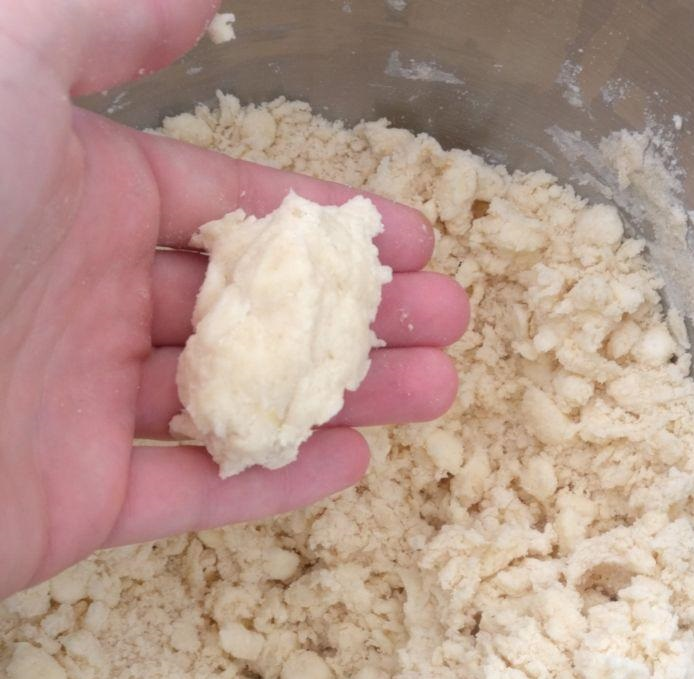
\includegraphics{images/pie-dough}}.

Gather all the crumbs together, just press them together, do not need the dough, into a square shape.
%
Cut it into four pieces, dust lightly with flour, and stack them together, to create some layers\sidenote{You can repeat this a couple or three times.}.
%
Wrap it\sidenote{Do you remember that reusable zip-lock bag?}, and put in the fridge for a at least a couple of hours.

\section{Baking}
Use some flour to open the dough with a rolling pin. 
%
Just put the dough in the tray and hit it with the filling, no need to bake before-hand. 
%
Egg-wash and sprinkle sugar on top.

Bake at $200^oC$ for about $30$ minutes, but keep and eye to not roast the top by putting it too close to the heat source. Ideally you have bottom heating as well.

\section{Experiments}
Instead of water, add something acidic, alcoholic, and possibly sweet to the dough. Great candidates are: Orange juice, White wine, and Cachaca.
%
The alcohol should evaporate during cooking, helping to keep the dough more crispy, while before cooking it helps to keep the dough "hydrated", making it easier to handle.
%
I guess the acid makes it harder to form gluten, resulting in a more flaky dough.

\section{Filling}

I personally like to cook apples, with a bit of corn starch (by eye), and seasoning, in very low heat, without steering, to not brake the apples, but to remove some moist before putting in the dough to bake\sidenote{Avoid soggy-bottoms. Amen!}.
%
It a great use for the zast and rest of the juice used to hydrate the dough.

Great candidates are peaches, and berries in general, mind if they have too much water.

Now, you can also use this dough to savoury pies, by simply reducing the amount of sugar by half.